\documentclass[xcolor = {dvipsnames}]{beamer}

\usetheme{Copenhagen}
\definecolor{verde}{rgb}{0, 0.80, 0}
\beamertemplatenavigationsymbolsempty
\addtobeamertemplate{navigation symbols}{}{%
    \usebeamerfont{footline}%
   \usebeamercolor[fg]{footline}%
    \hspace{1em}%
    \insertframenumber/\inserttotalframenumber
}
\title[QED of CNTs in cavity]{Study of quantum electrodynamics effects in cavity with carbon nanotubes \thanks{prof.Christophe Voisin, dr.Yannick Chassagneux}}


\author[Federico Rapisarda - LPENS]{Federico Rapisarda\\
Nano-optique group\\
LPENS}
\institute{
	Politecnico di Torino
	\and
	Universit\'{e} de Paris
}

\date[29 June 2021]{Paris, 29 June 2021}


\logo{%

\vspace{1mm} 
\includegraphics[width=2cm,height=1cm,keepaspectratio]{images/ens}%
  \hspace{\dimexpr\paperwidth-4cm-5pt}%
  
\includegraphics[width=2cm,height=1cm,keepaspectratio]{images/logo}%
}

%\logo{
%
\includegraphics[height=1cm]{images/ens}
%\hspace{125mm}
%
\includegraphics[height=1cm]{images/logo}
%}



\begin{document}
\frame{\titlepage}

\begin{frame}
\frametitle{Quantum information - the flying qubit}

How does a quantum network work?
\pause
\begin{itemize}
\item <2-> information processing in network's nodes $\rightarrow$ stationary qubits
\item <3-> decoherence-free information exchange between nodes $\rightarrow$ \alert{flying} qubits
\end{itemize}
\pause
Photons polarization can encode informations!\\
\end{frame}

%\begin{frame}{Towards quantum telecommunication}
%Polarization of photons can encode informations!\\
%Single photons sources:
%  \begin{itemize}
%	\item wavelength
%	\item count rate
%	\item polarization
%   \end{itemize}
%\end{frame}

\begin{frame}{Why CNTs?}
\begin{columns}

\begin{column}{0.6\textwidth}
Key requirements for quantum telecommunication:
\begin{itemize}
\item NIR emission
\item high emission efficiency
\end{itemize}
\end{column}

\begin{column}{0.4\textwidth}
 \begin{figure}
    \begin{overprint}
    \onslide<1> \centering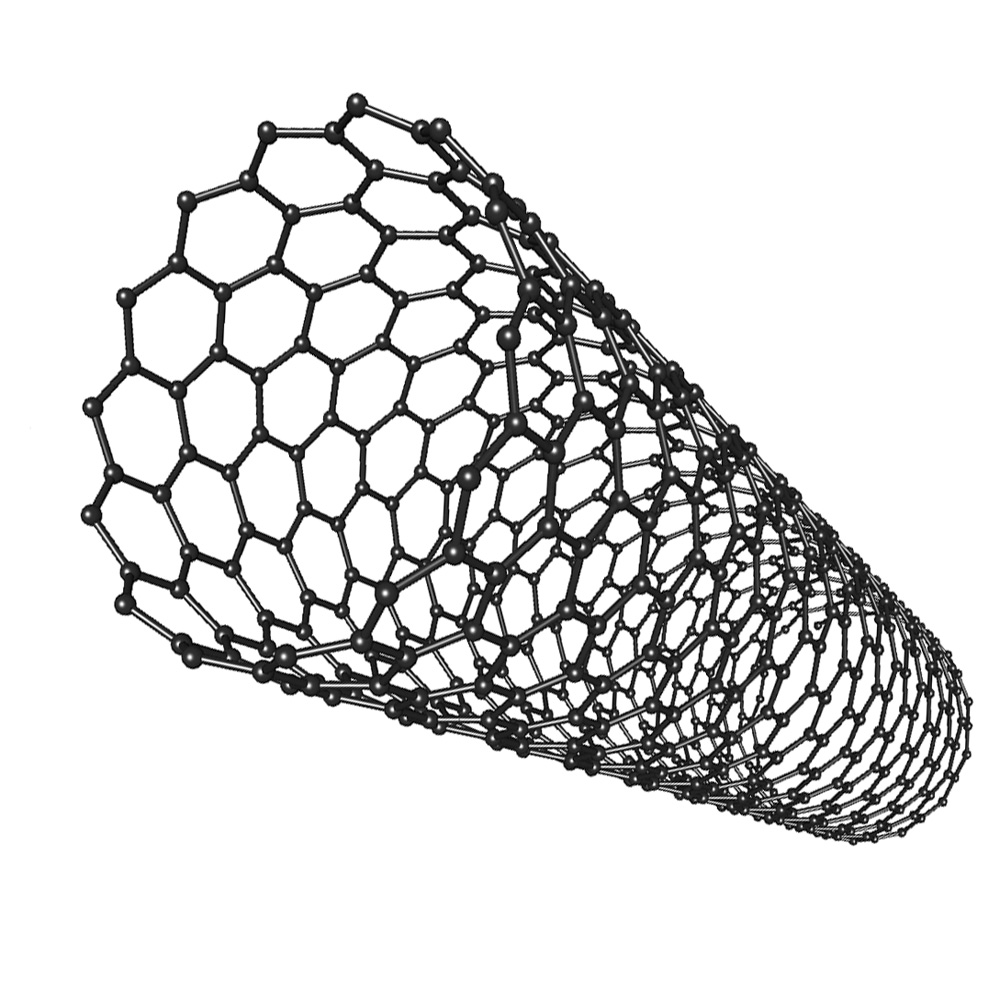
\includegraphics[width=1\textwidth]{images/CNT}
    \onslide<2>\centering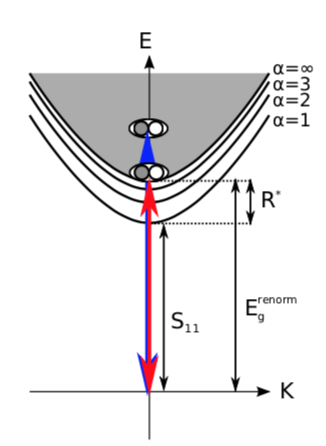
\includegraphics[width=.8\textwidth]{images/exciton}
    \end{overprint}
\end{figure}

\end{column}

\end{columns}
\end{frame}

\begin{frame}{The Nano-optique group work}
How to boost and control the emitting features of CNTs?\\
\begin{columns}
\begin{column}{0.6\textwidth}
Two parallel paths:
  \begin{itemize}
	\item <1-> modification of crystalline structures, environment and chemical features of materials
	\item <2-> photonic tools to reshape the emission properties of emitting material
  \end{itemize}
  \end{column}
  \begin{column}{0.4\textwidth}
  \centering
  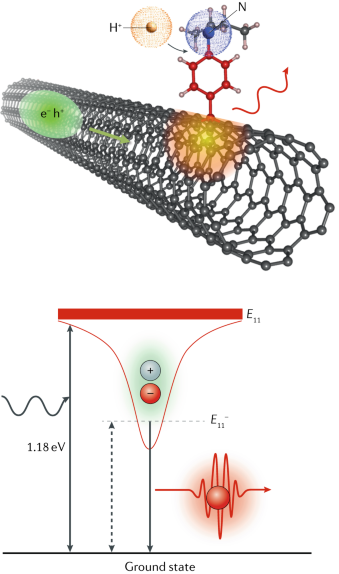
\includegraphics[width=.7\textwidth]{images/color}
  \end{column}
  \end{columns}
\end{frame}

\begin{frame}
	\frametitle{Carbon nanotubes in cavity}
	\begin{itemize}
	\item <1-> Fibered Fabry-Perot cavity
	\item  <1-> RT excitonic states exploitation for tuned optical transitions
	\end{itemize}
	\hspace{0.5cm}
	\vspace{-0.5cm}

	\begin{figure}[h!]
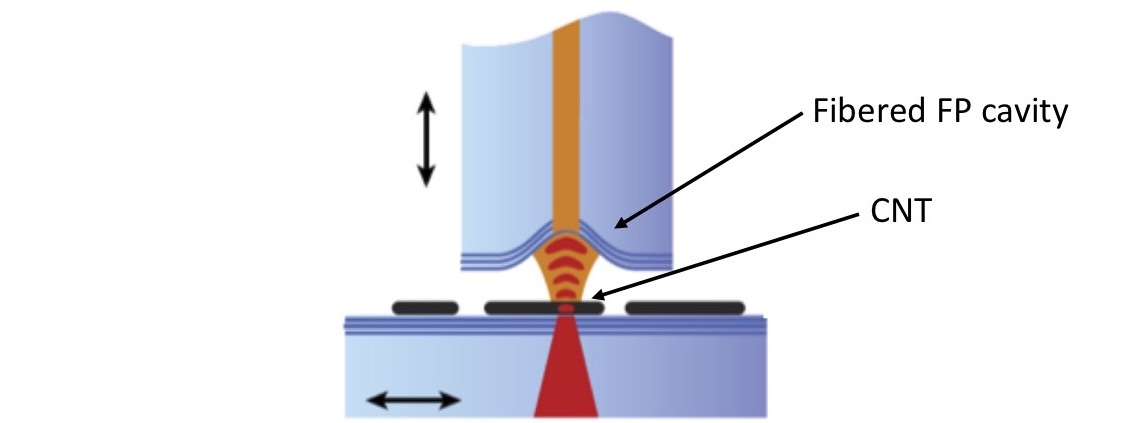
\includegraphics[width=.9\textwidth]{images/cavity}
	\end{figure}
	\emph{\scriptsize Collaboration with Jacob Reichel, LKB}
	\end{frame}

\begin{frame}{Carbon nanotubes in cavity}

\begin{columns}
\begin{column}{0.6\textwidth}
\begin{itemize}
	\item <1-> Fibered Fabry-Perot cavity. \textcolor{verde}{Spectral} and \textcolor{Cerulean}{spatial} coupling of CNTs
\end{itemize}
\vspace{-3mm}
  \begin{figure}
  \centering
  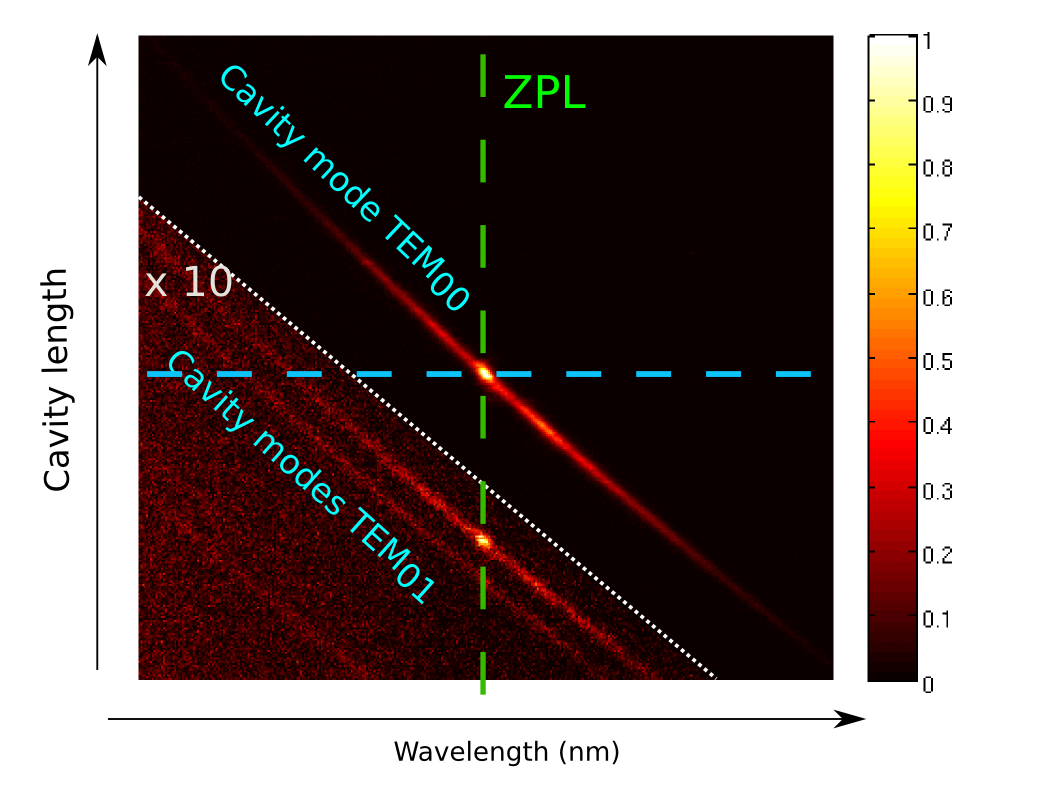
\includegraphics[width=1\textwidth]{images/match}
  \end{figure}
  \end{column}
  \begin{column}{0.4\textwidth}
   \begin{figure}
  \centering
  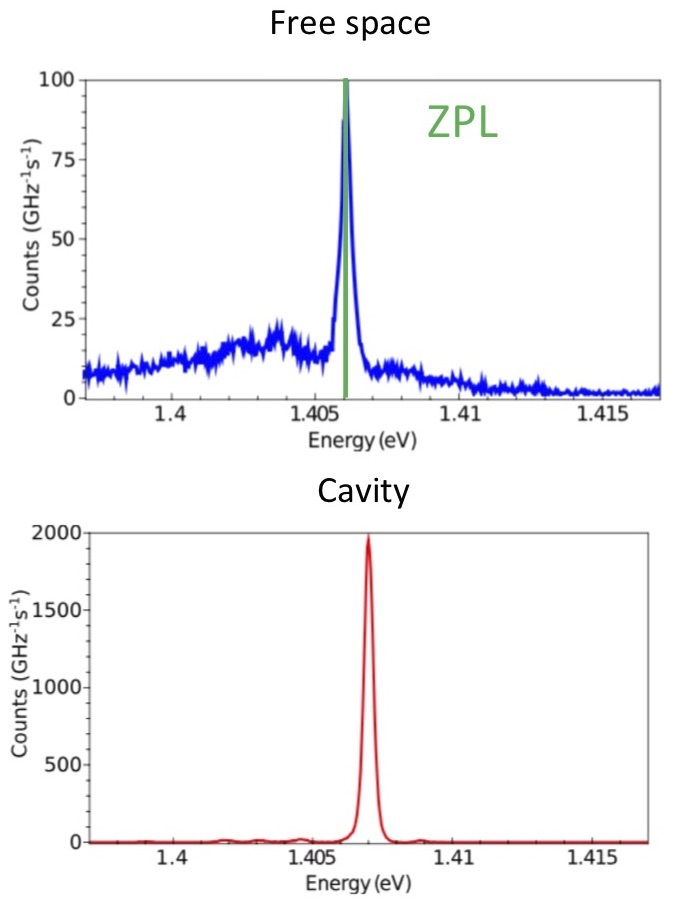
\includegraphics[width=.8\textwidth]{images/ZPL}
  \end{figure}
  \end{column}
  \end{columns}
\end{frame}

\begin{frame}{The deep-subwavelngth regime}
	\begin{figure}[h!]
		\centering
    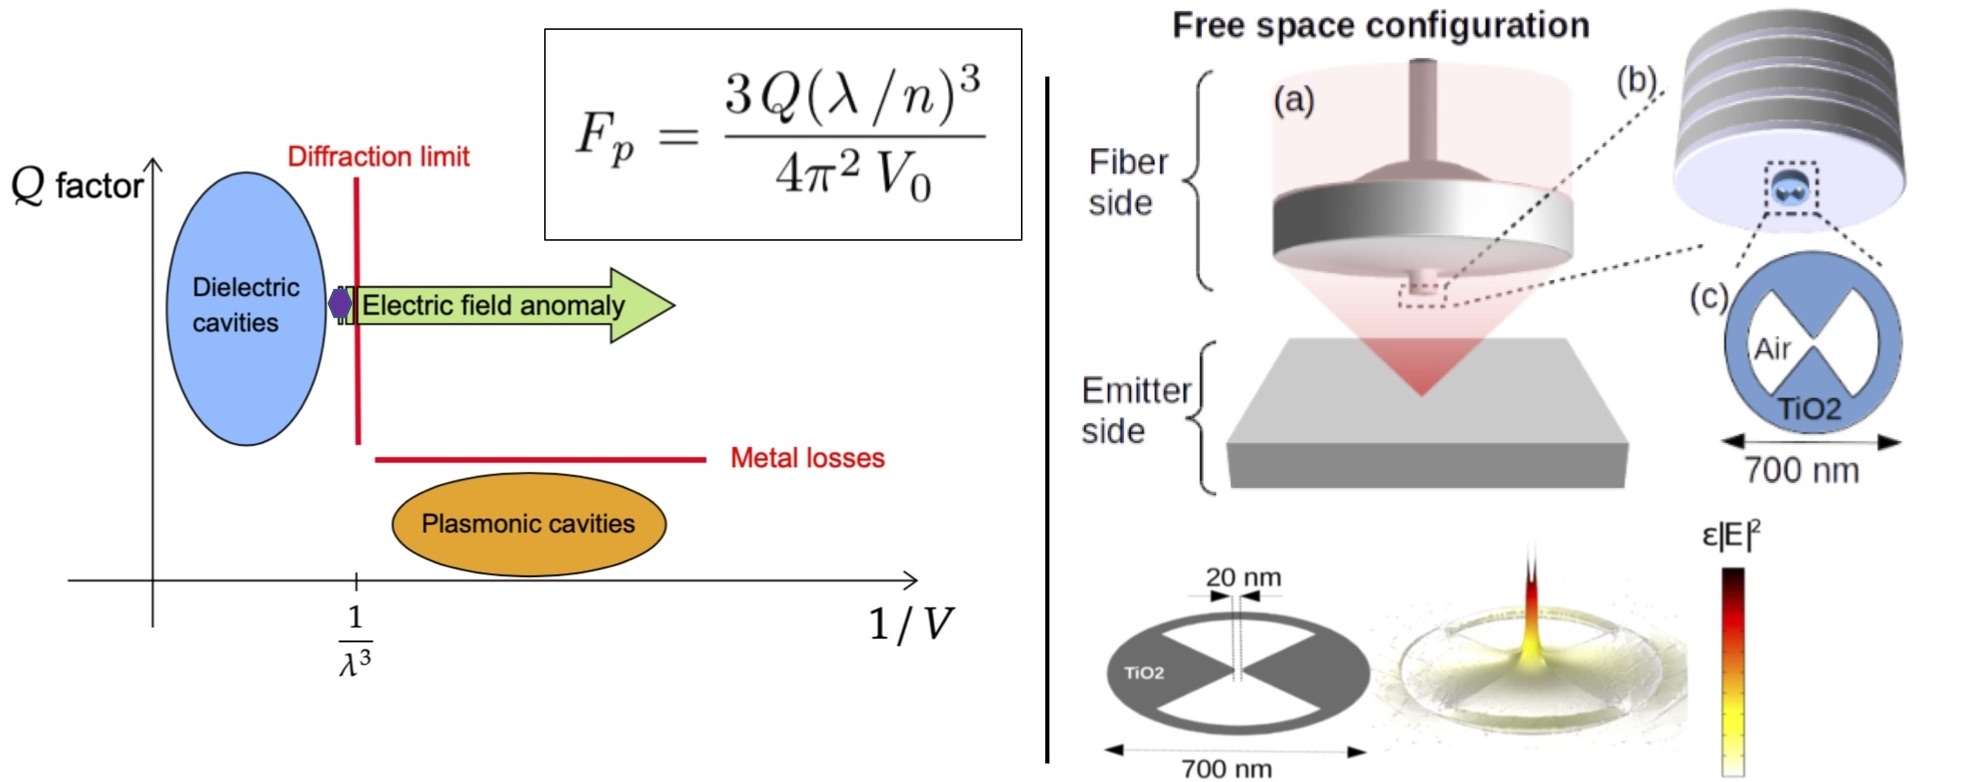
\includegraphics[width=1\textwidth]{images/fine}
	\end{figure}
\end{frame}



\begin{frame}[t]{Sub-diffraction image of the intensity map}
\begin{columns}
\column{0.4\textwidth}

\centering "Diverging" optical field

\begin{figure}[h!]
\centering
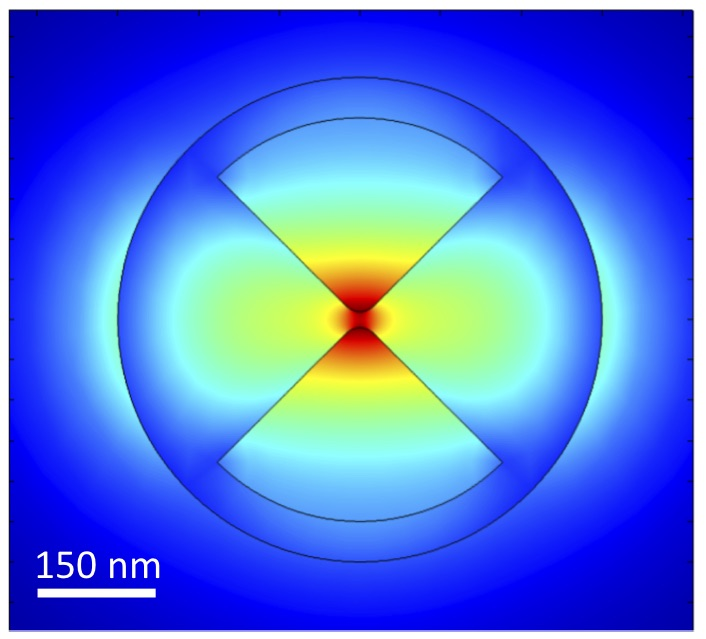
\includegraphics[width=1\textwidth]{images/intensity}
\end{figure}
\centering
EM field finite element simulation
\column{0.6\textwidth}
\end{columns}
\end{frame}

\begin{frame}{Sample preparation}
\begin{columns}
\column{0.4\textwidth}
\centering
Dielectric nano-antenna
\begin{figure}[h!]
\centering
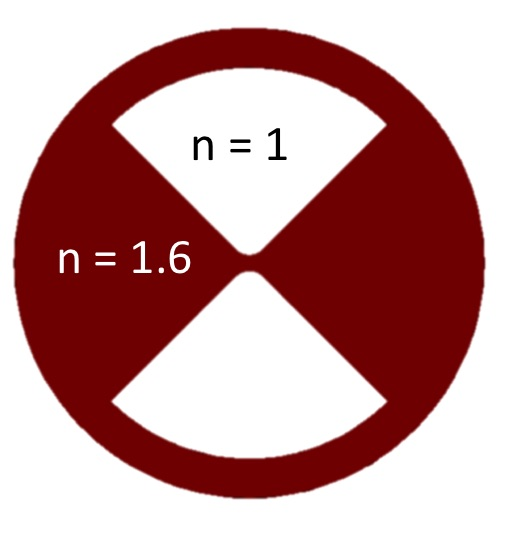
\includegraphics[width=1\textwidth]{images/antenna}
\end{figure}
\column{0.6\textwidth}
\pause
\centering
Sample fabrication
\begin{figure}[h!]
\centering
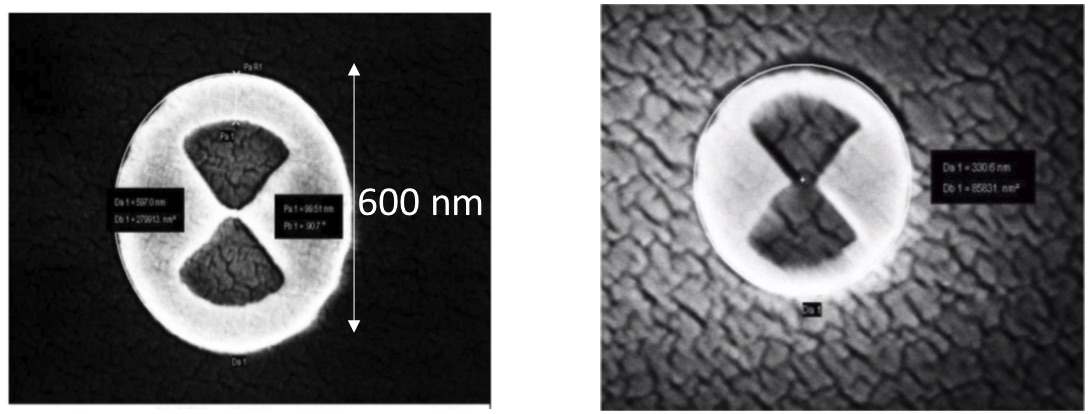
\includegraphics[width=1\textwidth]{images/compare}
\end{figure}
\centering
\hspace{-1cm}nano-bridge \qquad nano-gap
\end{columns}
\end{frame}


\begin{frame}{Sample characterization}
	\begin{figure}
    \begin{overprint}
    \onslide<1> \centering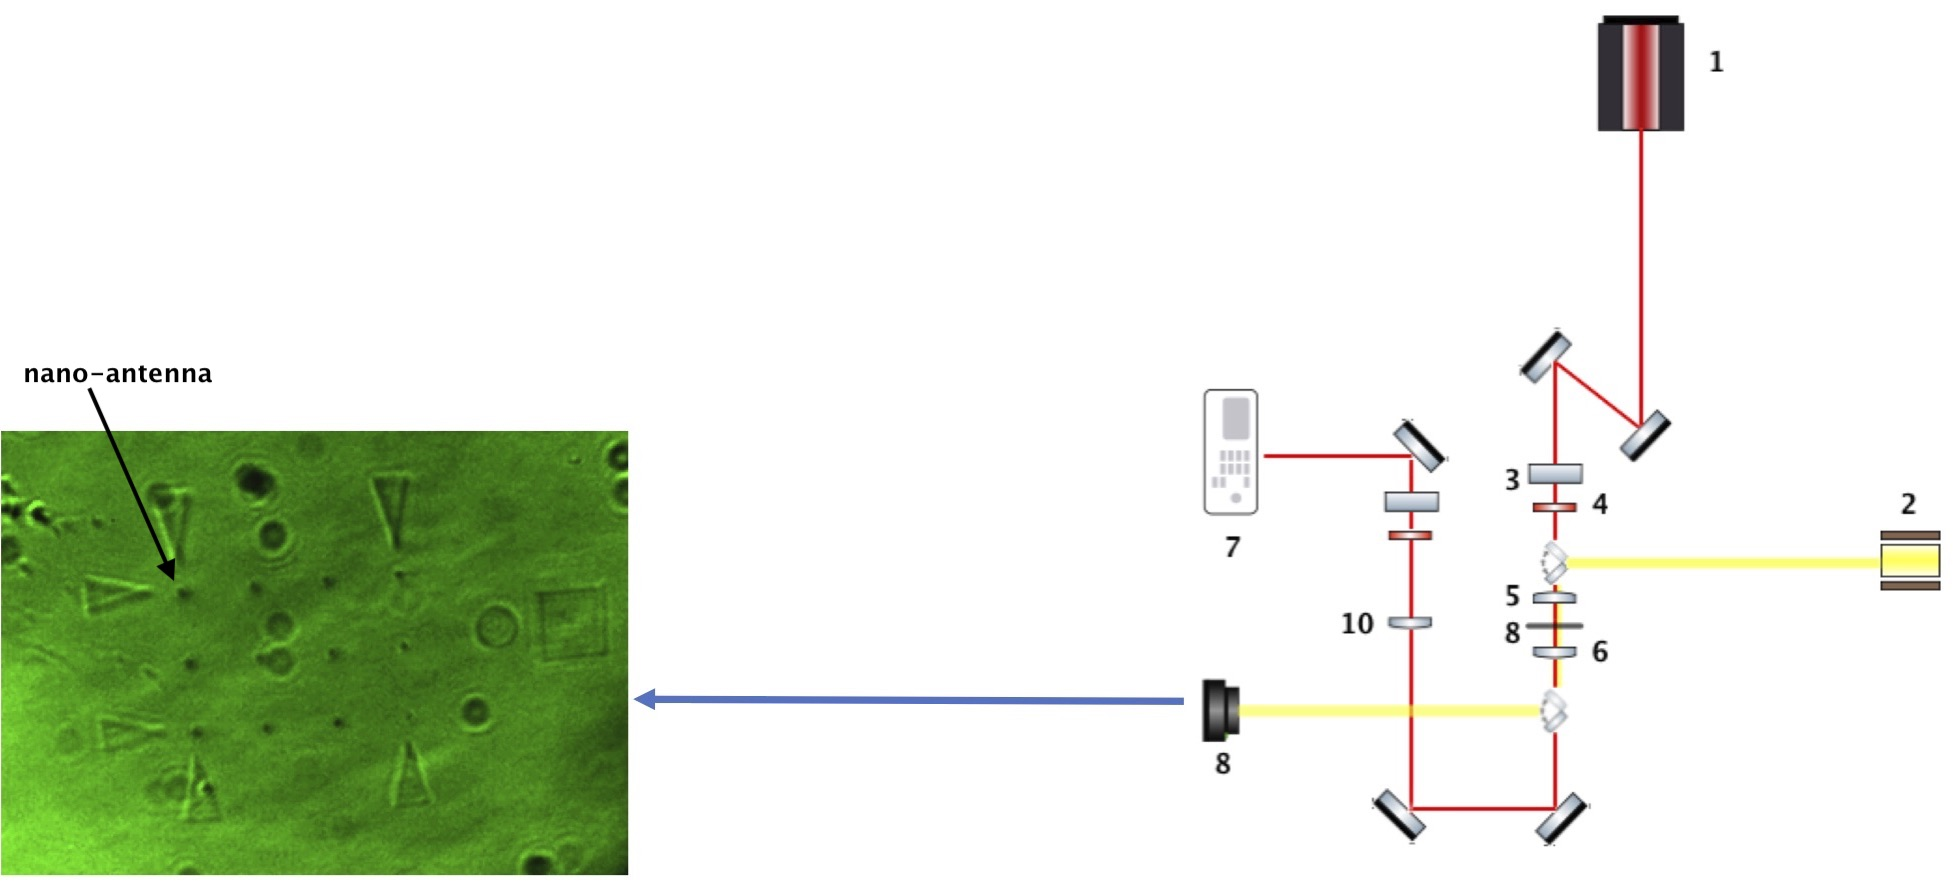
\includegraphics[width=1.05\textwidth]{images/setup1}
    \onslide<2>\centering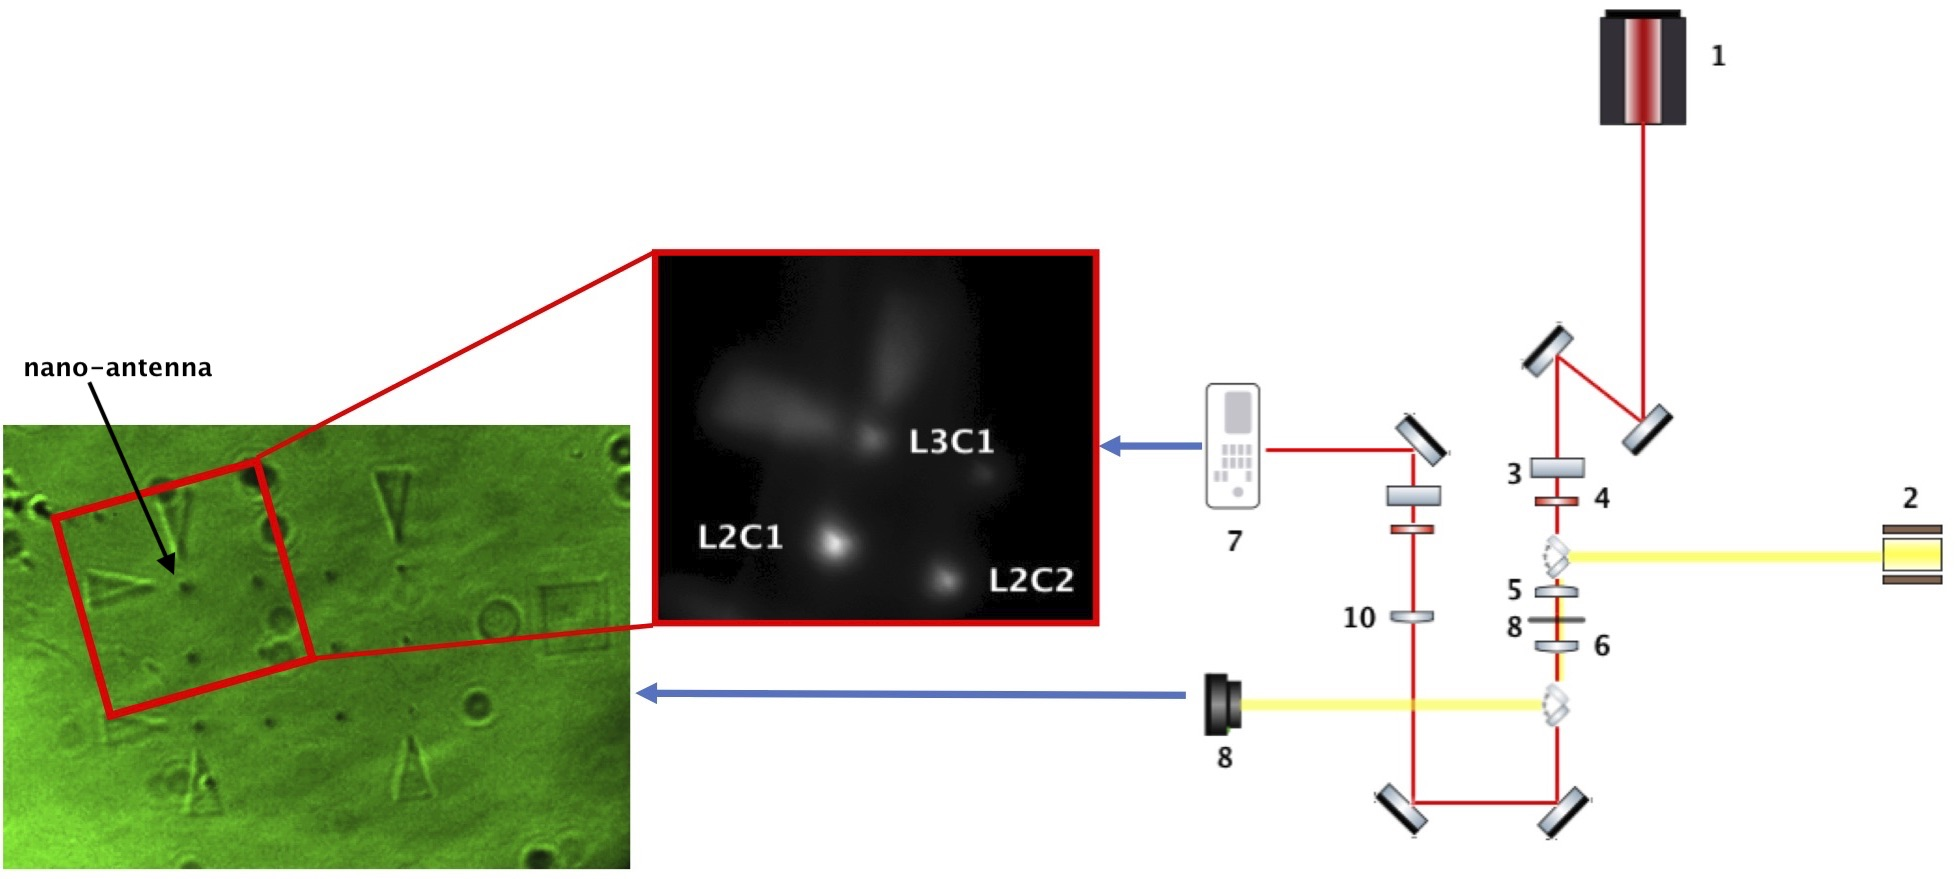
\includegraphics[width=1.05\textwidth]{images/setup2}
    \end{overprint}
\end{figure}
\end{frame}

\begin{frame}[t]{Polarization measurements}
	\begin{figure}[h!]
	\centering
	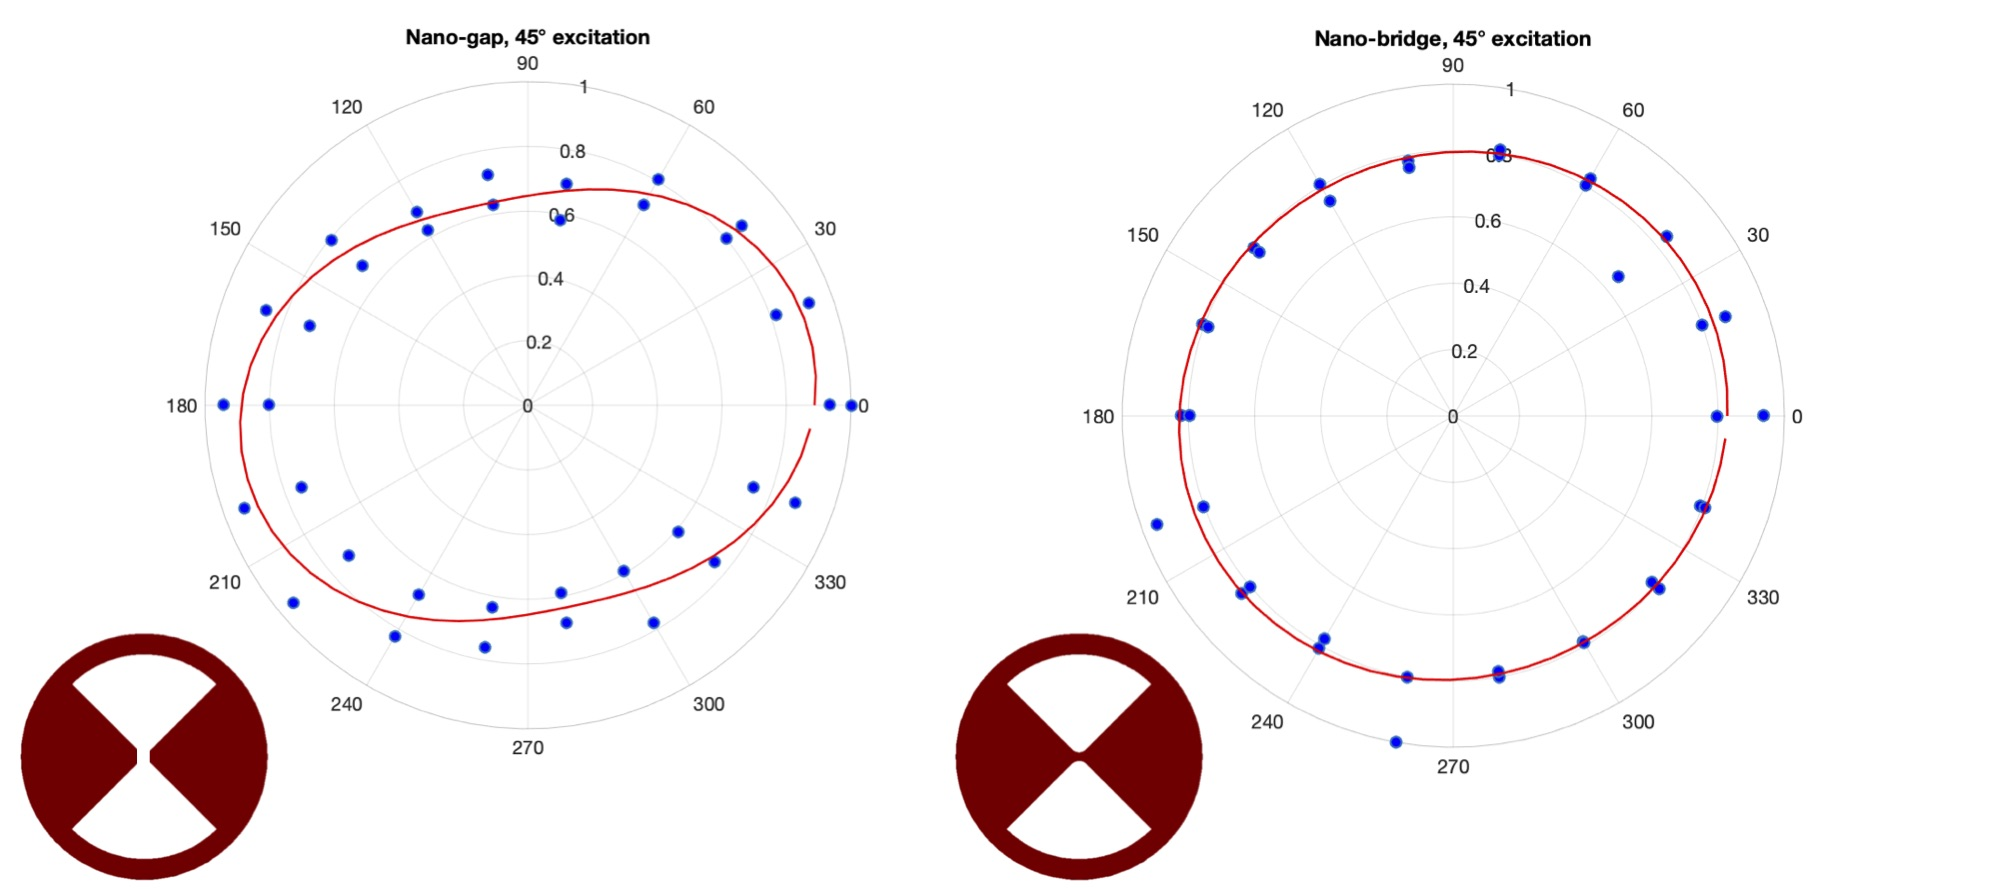
\includegraphics[width=1.07\textwidth]{images/polarization}
	\end{figure}
\end{frame}

\begin{frame}{Sub-diffraction image of the intensity map}
\begin{columns}
\column{0.4\textwidth}
\centering "Diverging" optical field
\begin{figure}[h!]
\centering
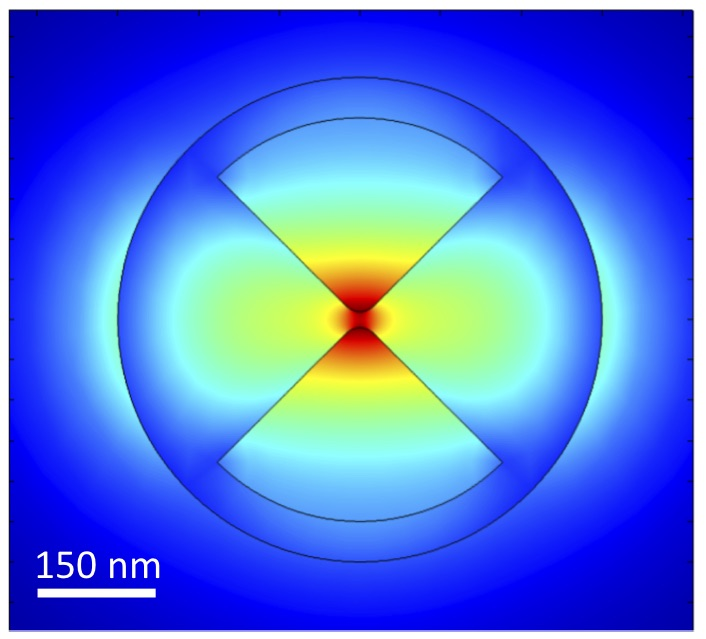
\includegraphics[width=1\textwidth]{images/intensity}
\end{figure}
\centering
EM field finite element simulation
\column{0.6\textwidth}
\end{columns}
\end{frame}

\begin{frame}{Super-resolution technique}
	\begin{figure}[h!]
	\centering
	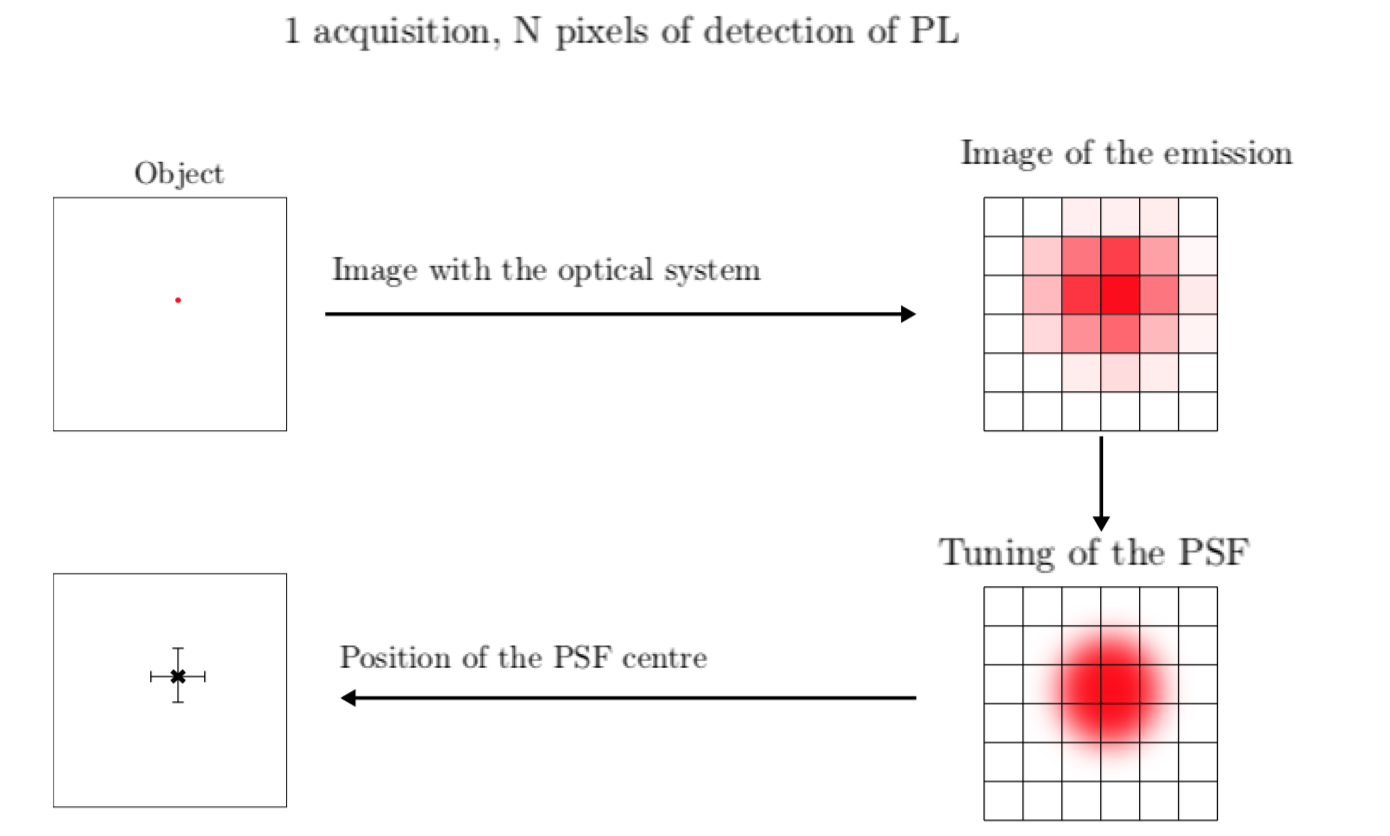
\includegraphics[width=.9\textwidth]{images/SR}
	\end{figure}
\end{frame}



\begin{frame}{Super-resolution technique}
	\begin{figure}
		\begin{overprint}
		\onslide<1> \centering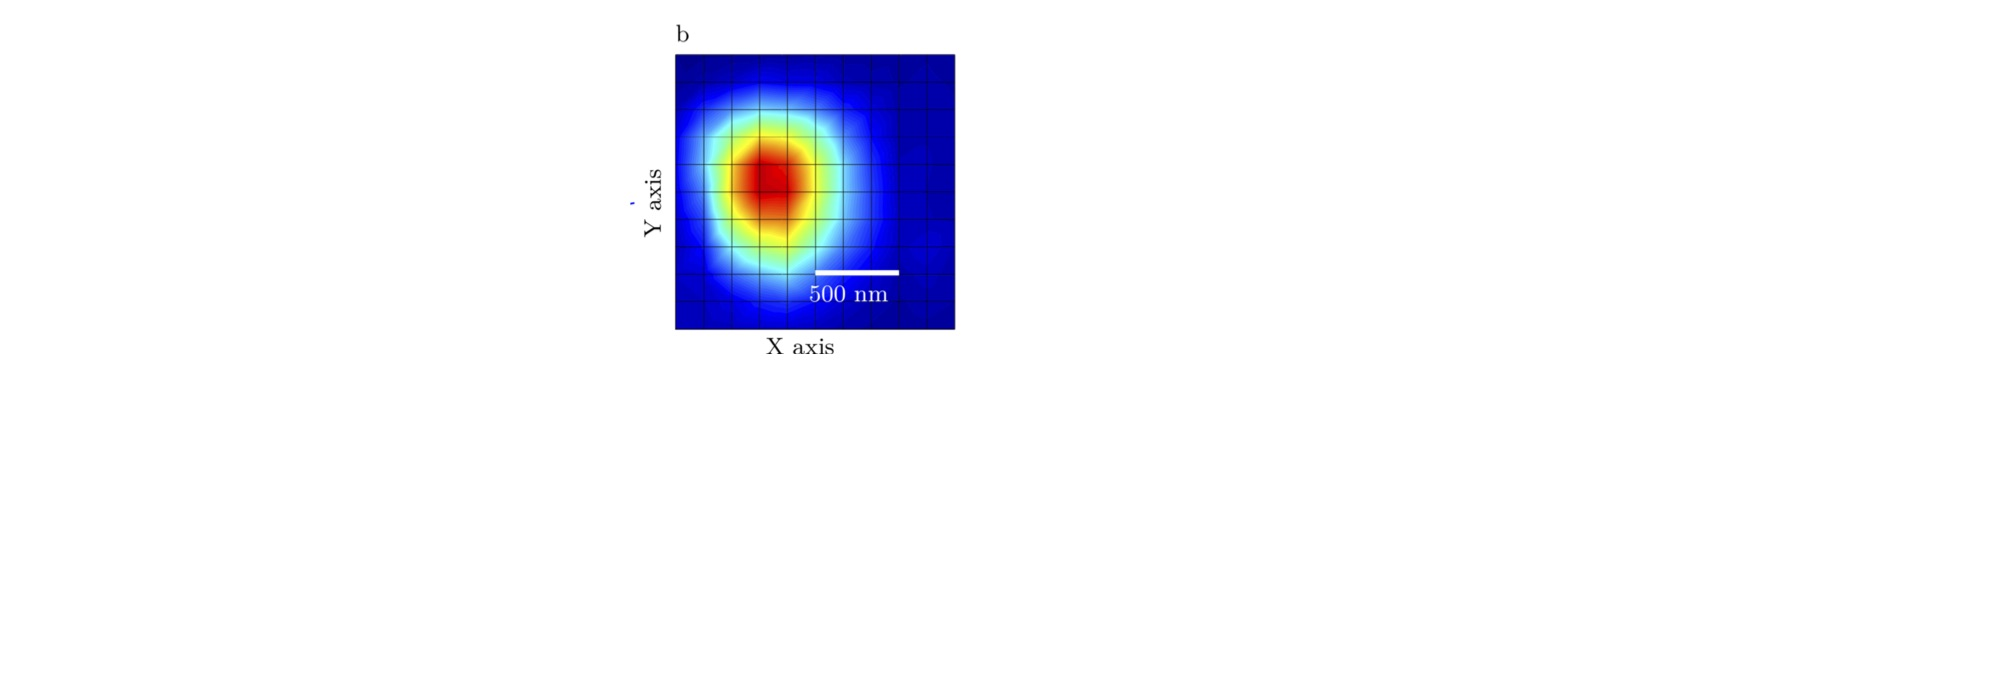
\includegraphics[width=1.05\textwidth]{images/s1}
		\onslide<2>\centering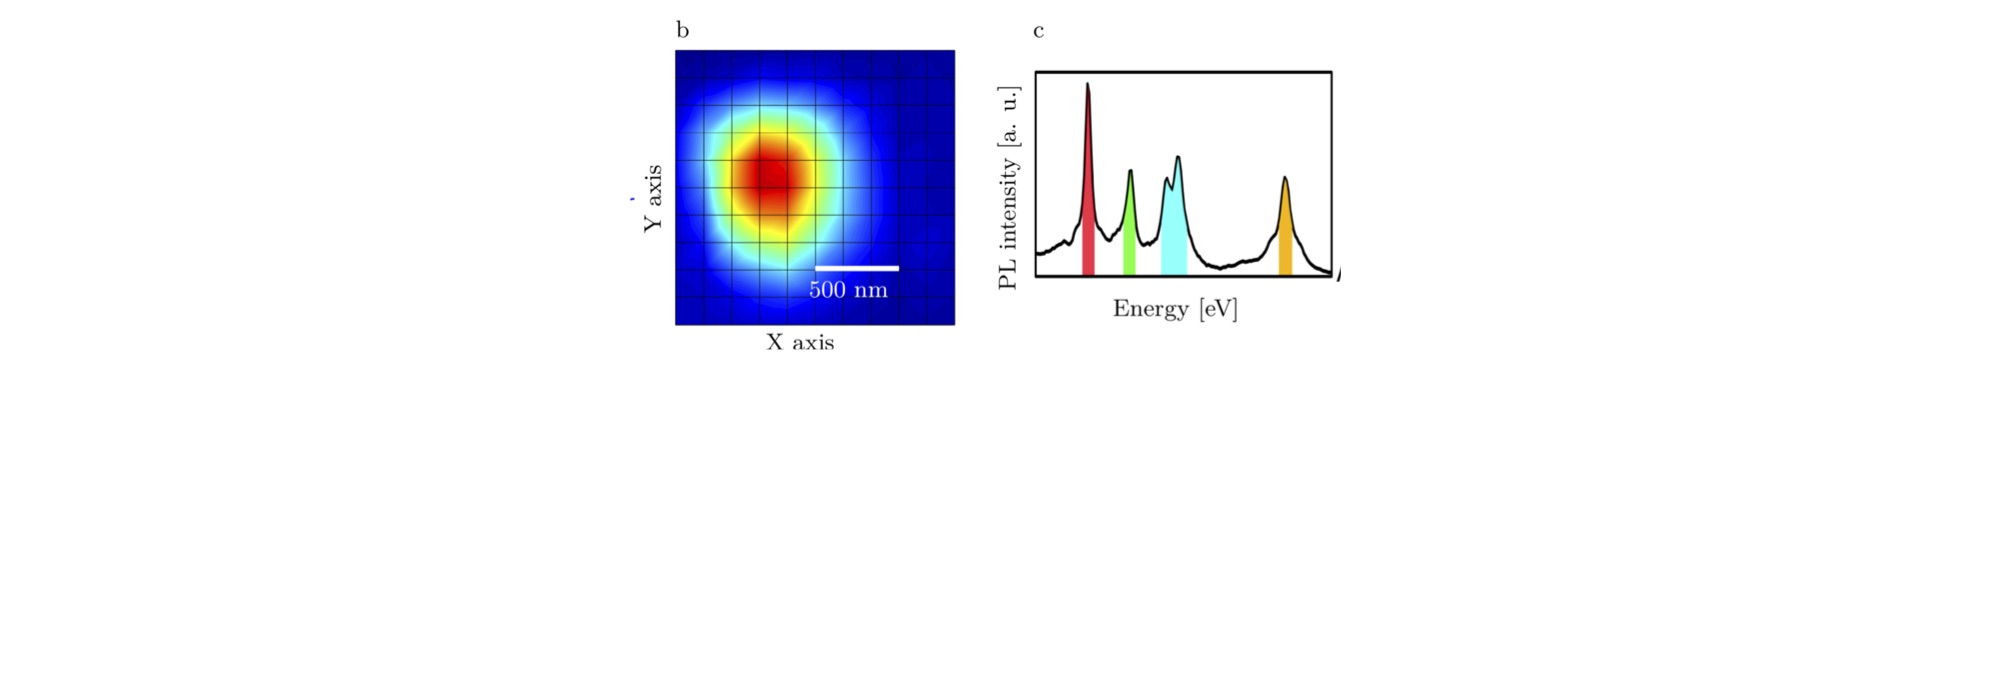
\includegraphics[width=1.05\textwidth]{images/s2}
		\onslide<3> \centering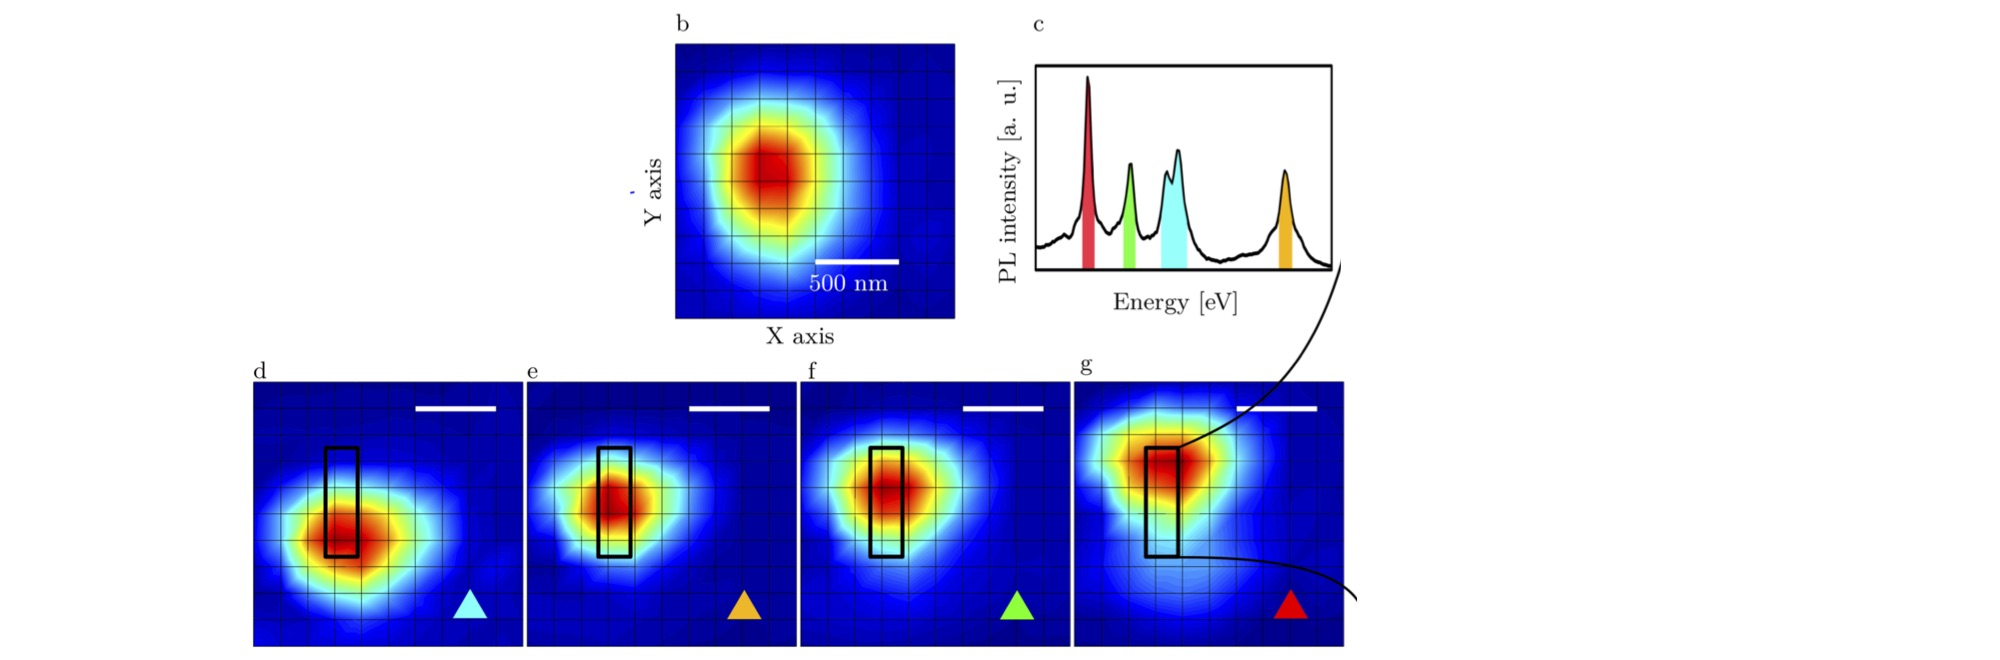
\includegraphics[width=1.05\textwidth]{images/s3}
		\onslide<4>\centering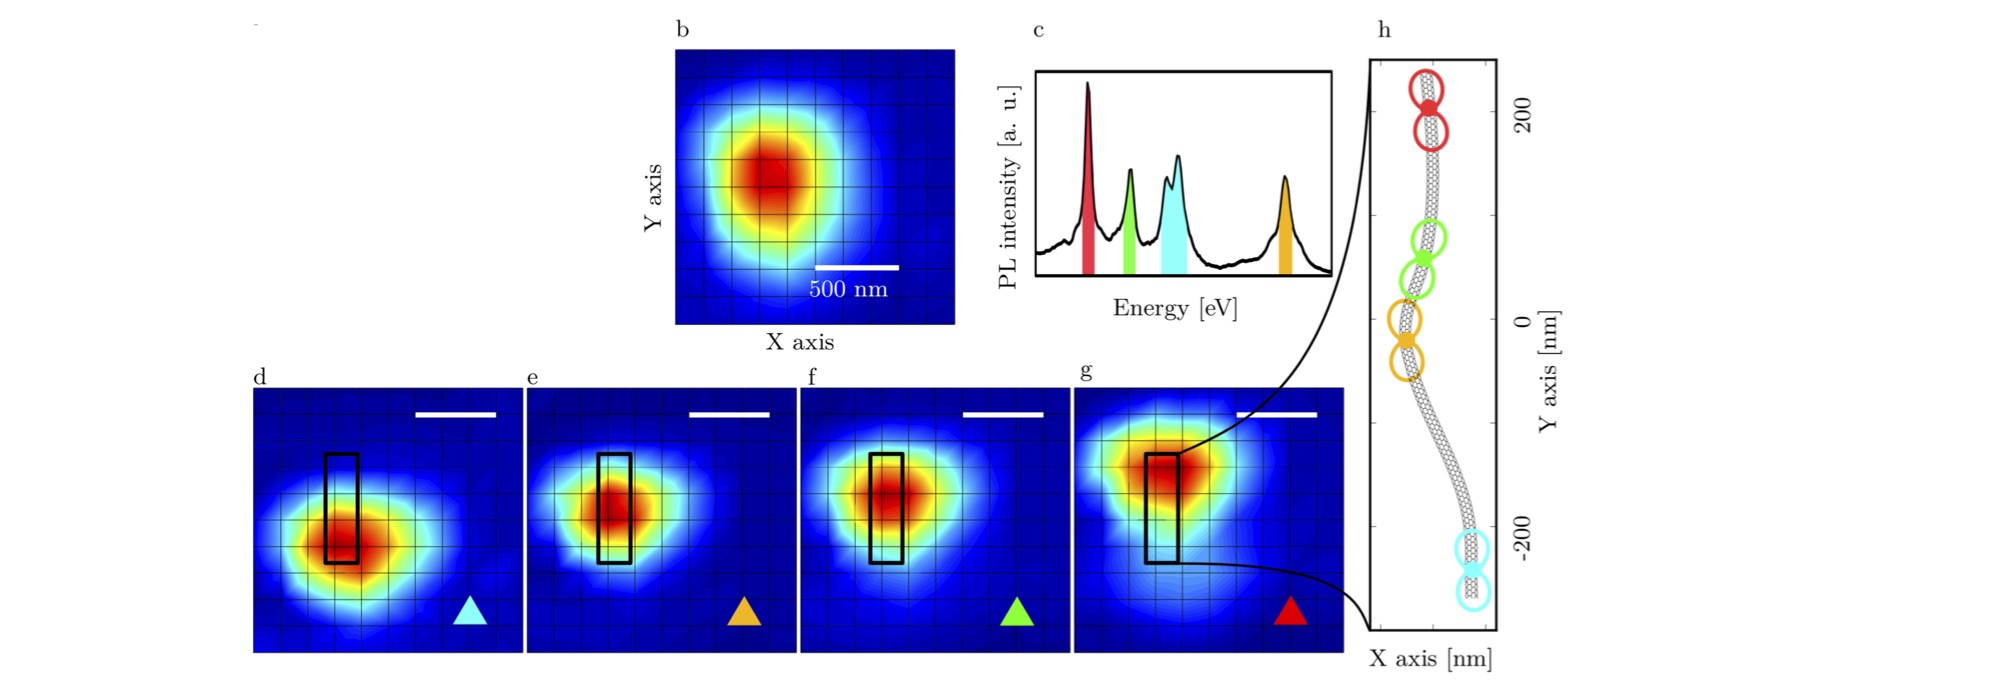
\includegraphics[width=1.05\textwidth]{images/s4}
		\end{overprint}
	\end{figure}
	\tiny C. Raynaud, T. Claude, A. Borel, M. Amara, A. Graf, et al.. Superlocalization of Excitons in Carbon Nanotubes at Cryogenic Temperature. Nano Letters, American Chemical Society, 2019, 19 (10), pp.7210-7216.
\end{frame}

\begin{frame}{Organic dye for super-resolution}
	\begin{figure}
		\begin{overprint}
		\onslide<1> \centering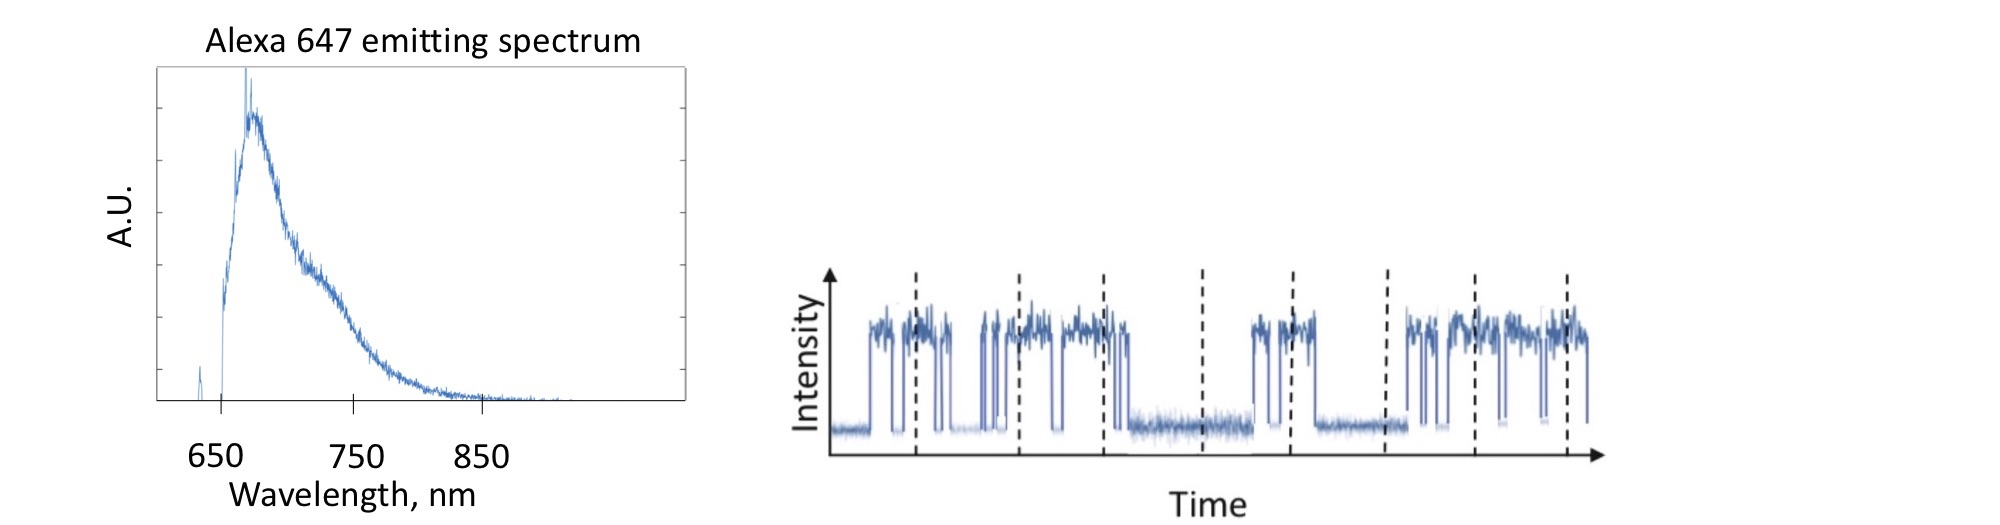
\includegraphics[width=1.15\textwidth]{images/alexa1}
		\onslide<2>\centering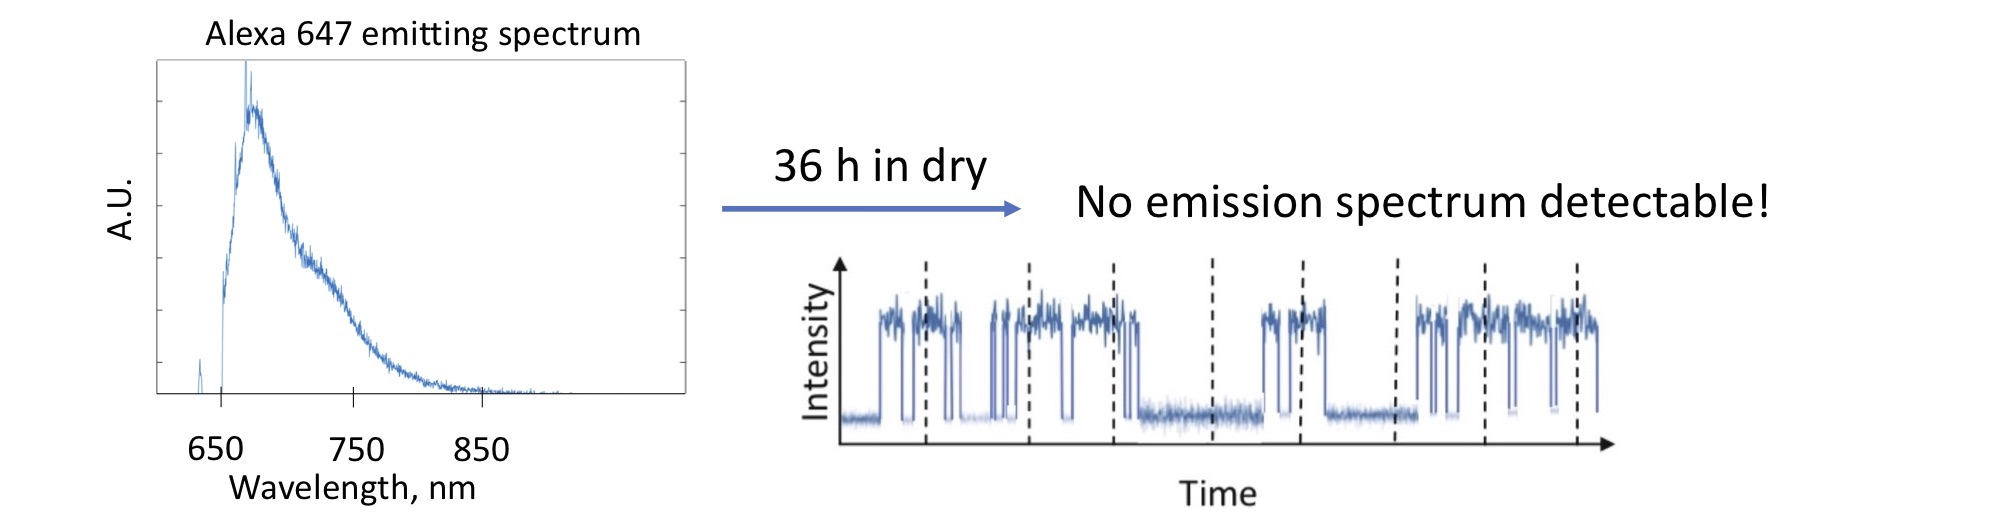
\includegraphics[width=1.15\textwidth]{images/alexa2}
		\end{overprint}
		\end{figure}
		\begin{itemize}
		\item <2-> New route: Alexa + polystyrene matrix
		\end{itemize}
\end{frame}

\begin{frame}[t]{HSQ for super-resolution}
\vspace{1cm}
	\begin{figure}
		\begin{overprint}
		\onslide<1> \centering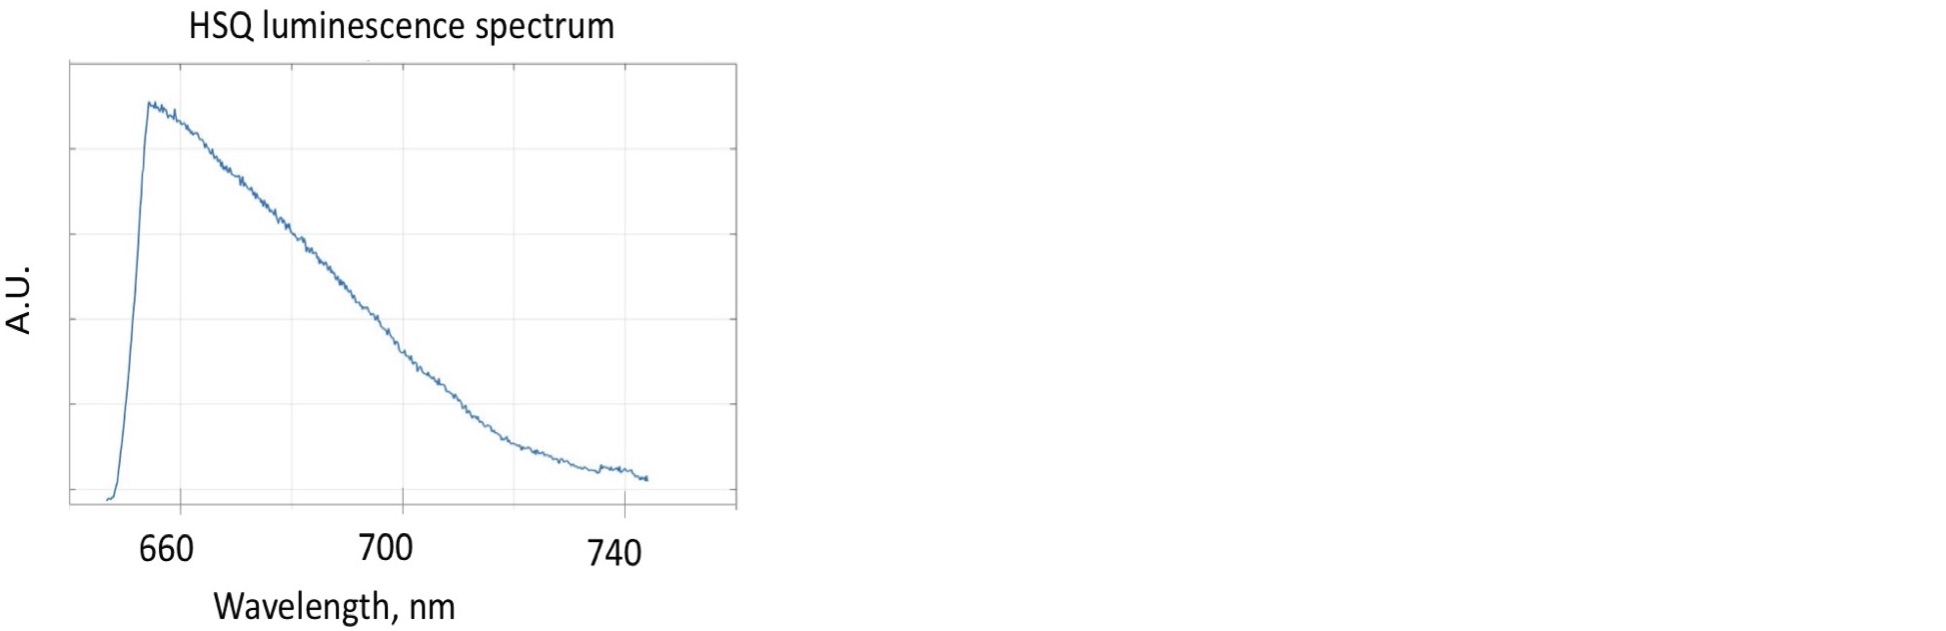
\includegraphics[width=1\textwidth]{images/hsq}
		\onslide<2>\centering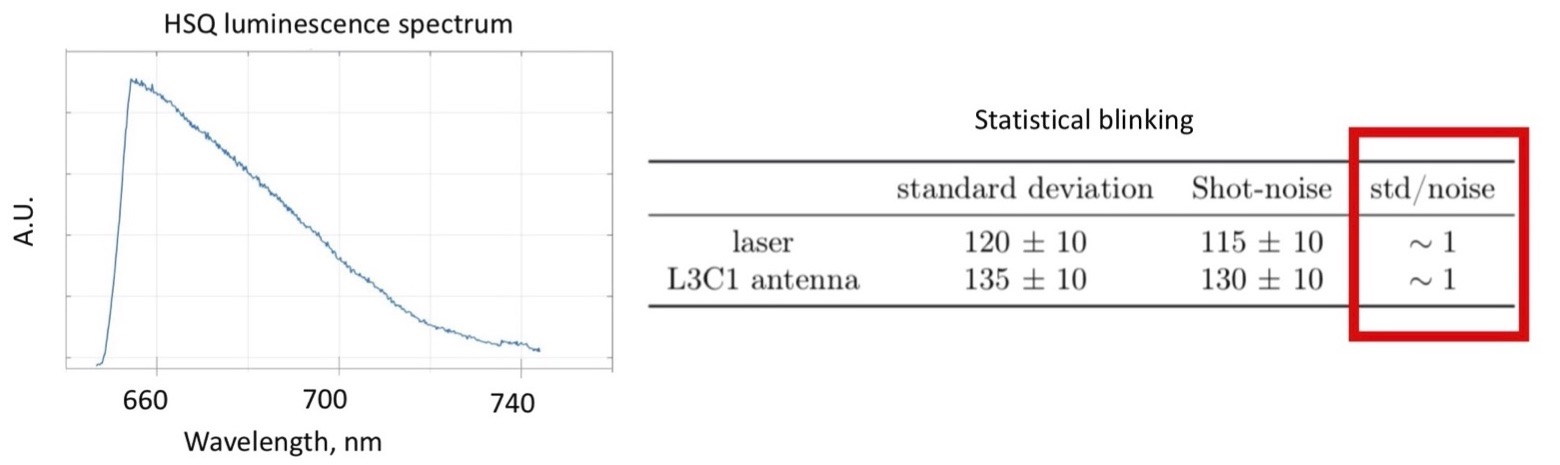
\includegraphics[width=1\textwidth]{images/hsq2}
		\end{overprint}
		\end{figure}
\end{frame}

\begin{frame}{My internship so far}
\begin{itemize}
\item Coupling of CNTs in cavity (in collaboration with PhD student Antoine Borel)
\item Nano-antenna design and production
\item Setup design and building
\item Preliminary steps towards super-resolution measurements
\end{itemize}
\end{frame}

\begin{frame}{Towards a new physics}
\begin{figure}
    \centering

    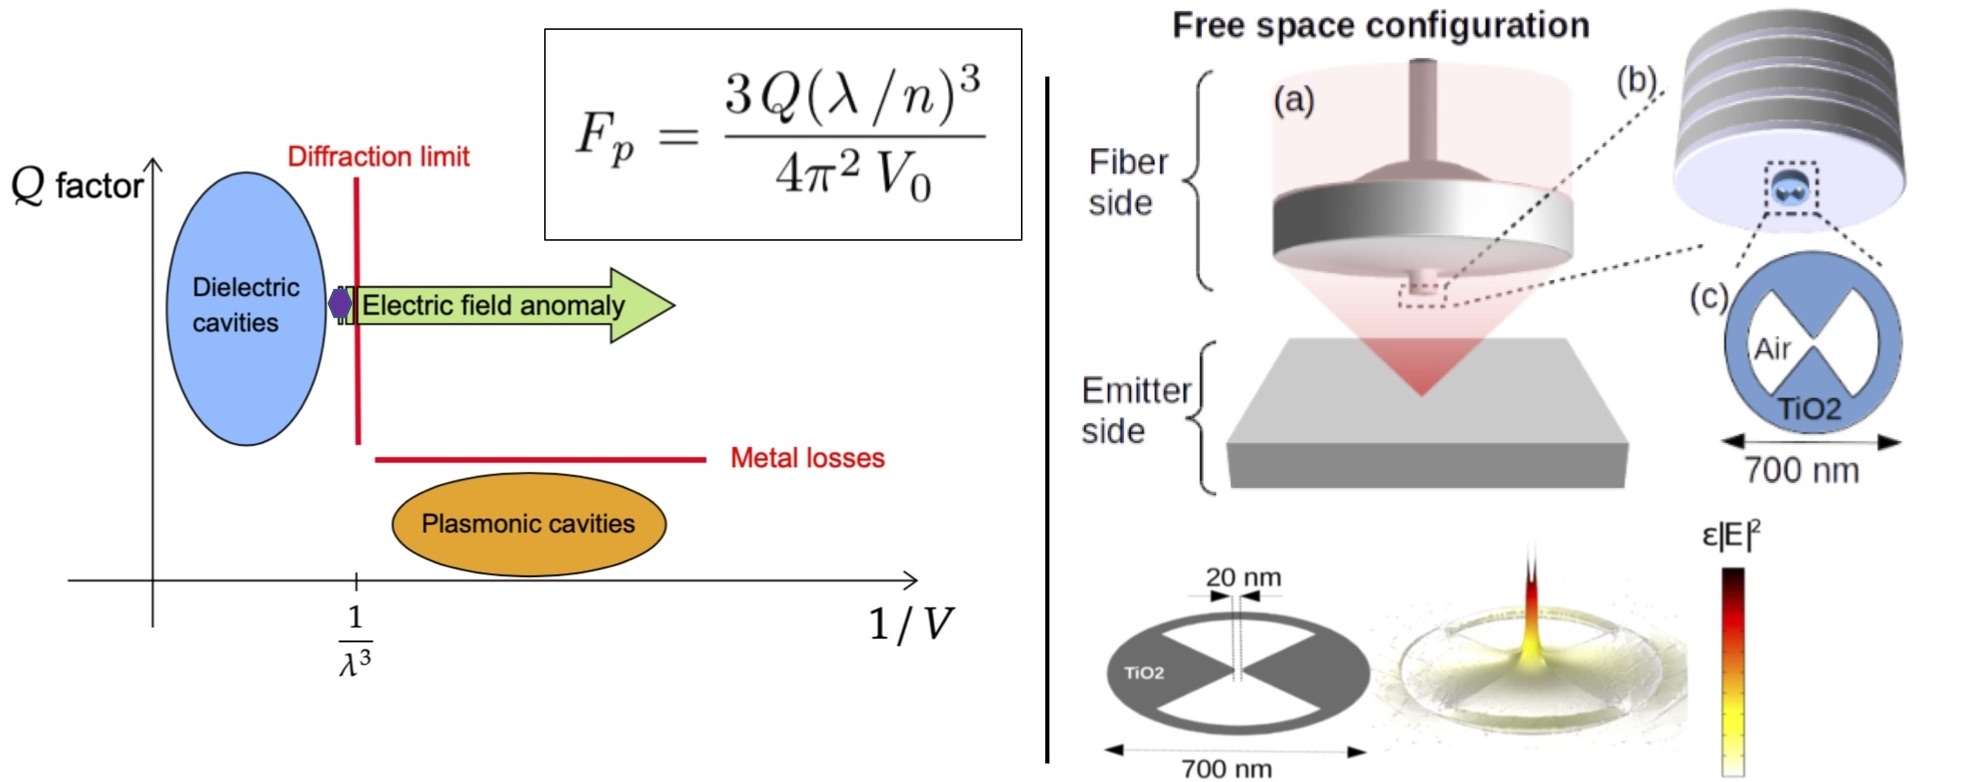
\includegraphics[width=1\textwidth]{images/fine}
    \end{figure}
\end{frame}
\begin{frame}
\frametitle{Acknowledgments}
The Nano-optique group:\\ 
\vspace{1mm}
prof. C.Voisin, C.Diederichs, E.Baudin, dr. Y.Chassagneux \\
\vspace{1mm}
PhD Antoine Borel, Raouf Amara, Zakaria Said, Marin Tharrault
\end{frame}

\begin{frame}
\centering
\Large Thank you for your attention
\end{frame}

\begin{frame}
\vspace{-1cm}
	\begin{figure}[h!]
	\centering
	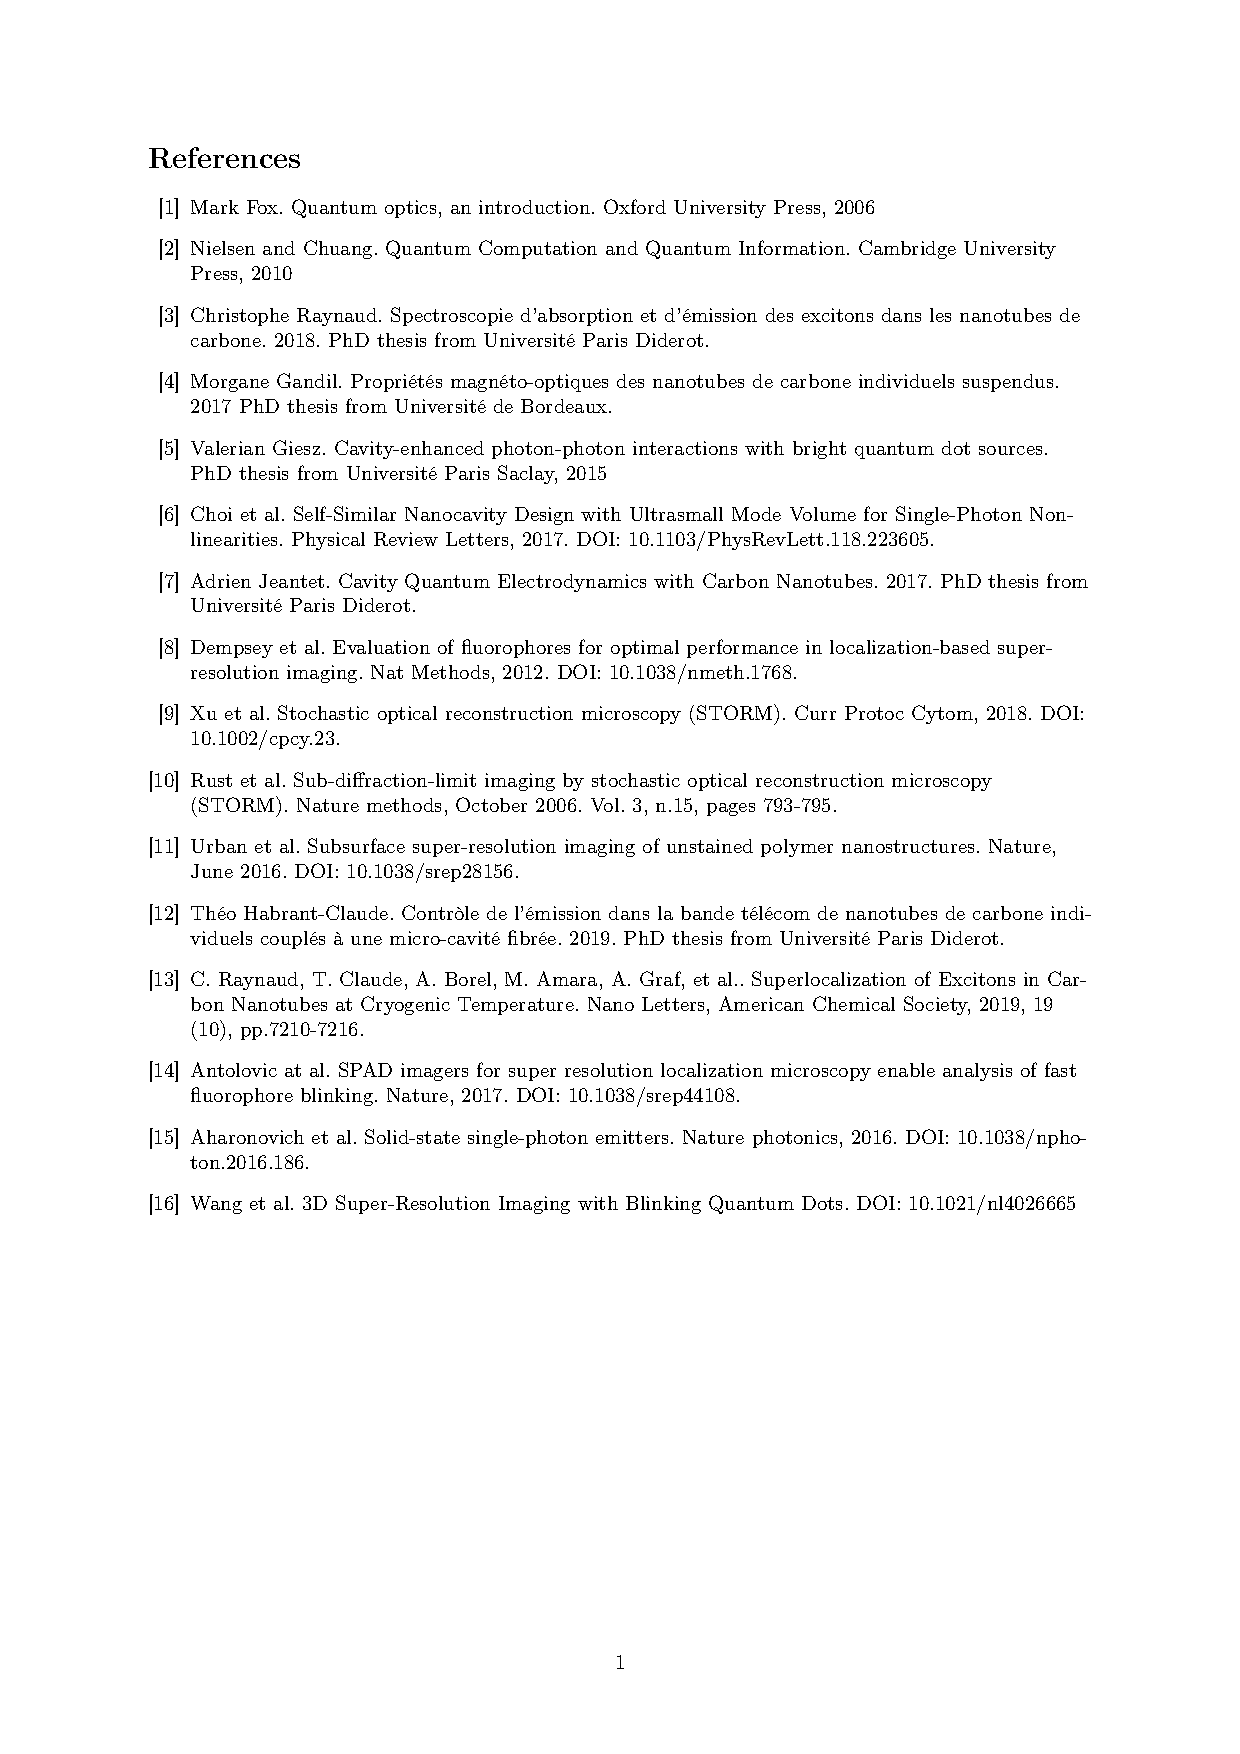
\includegraphics[width=.9\textwidth]{images/Bibliography}
	\end{figure}
\end{frame}

\begin{frame}{Isolation of single antenna}
\begin{figure}
\centering
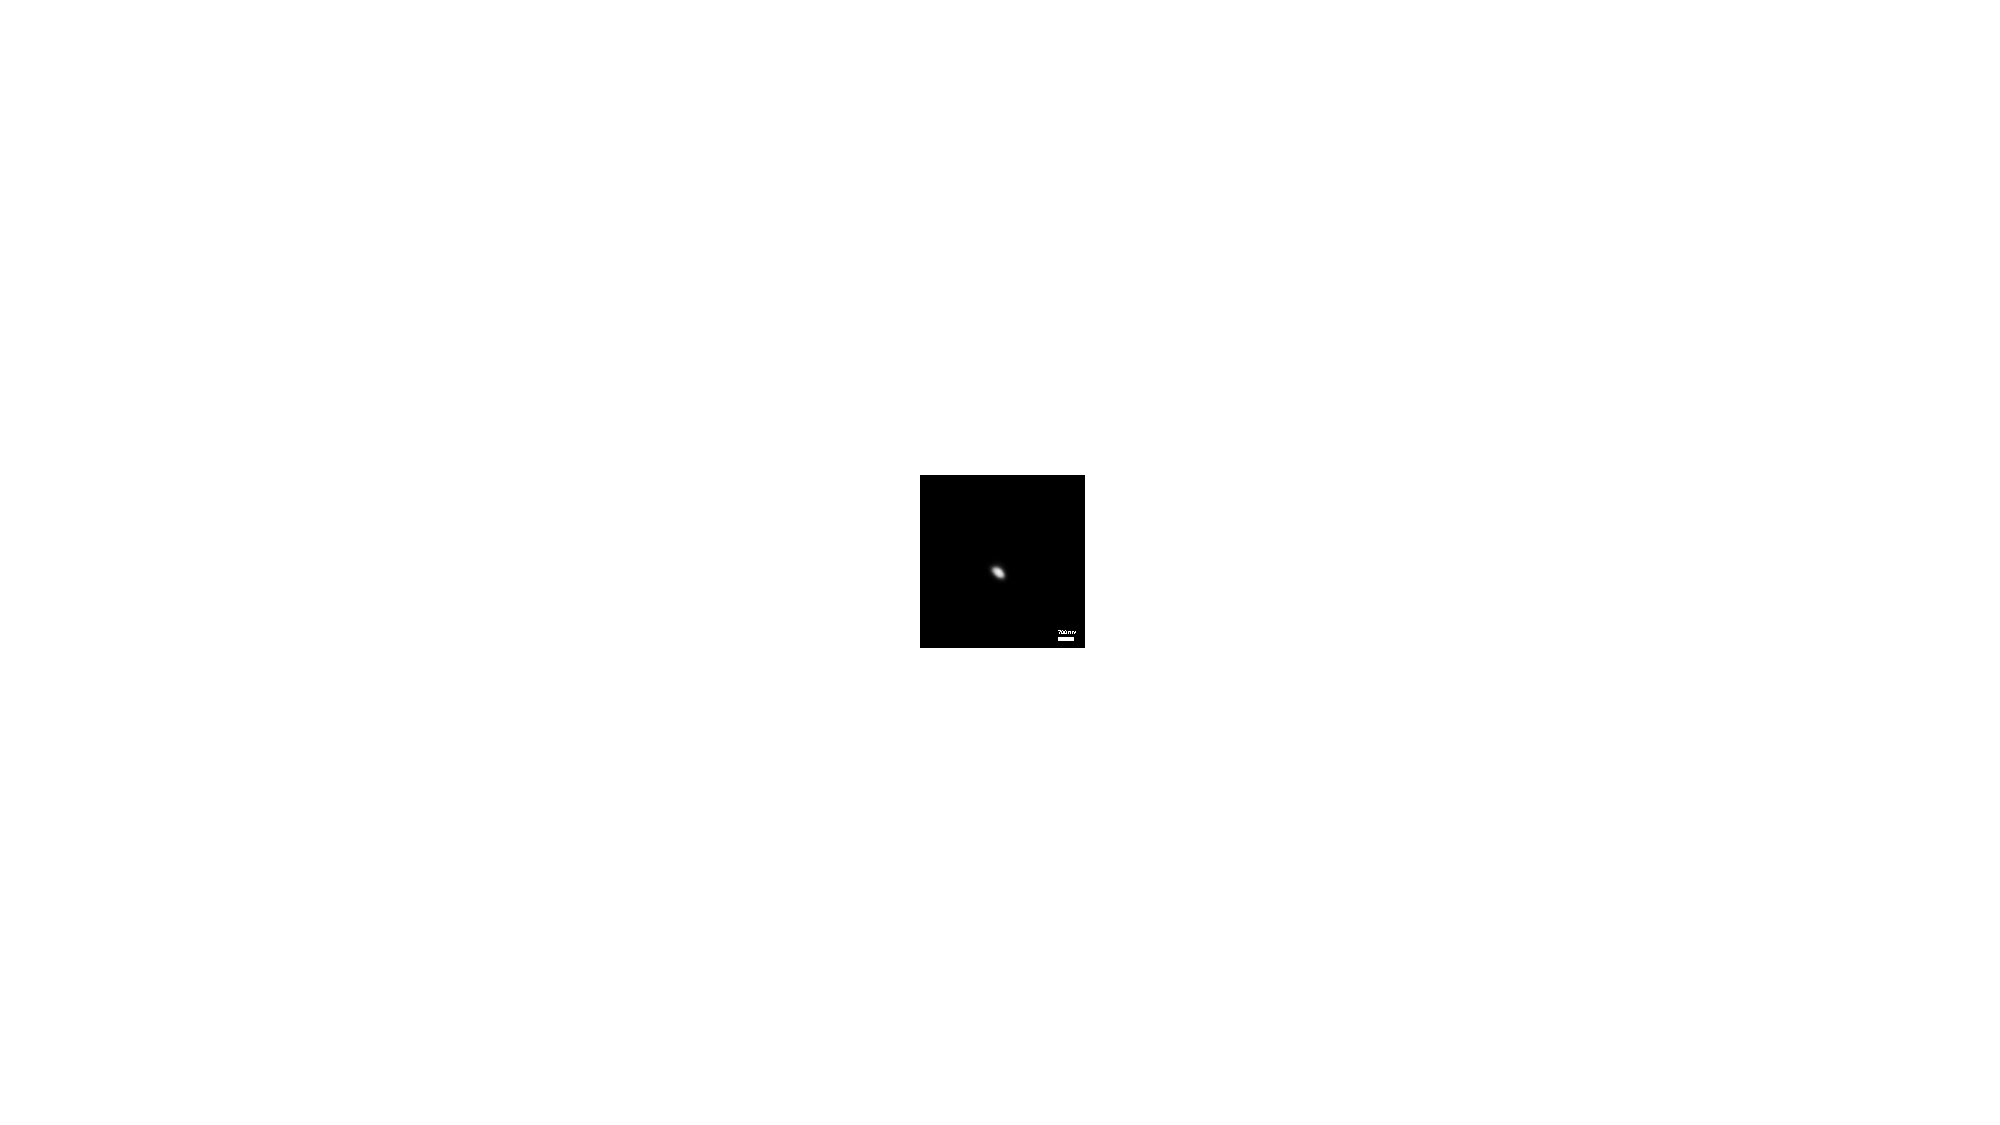
\includegraphics[width=.4\textwidth]{images/antenna_2}
\end{figure}
\end{frame}

\begin{frame}{The strong coupling regime}
\begin{figure}
\centering
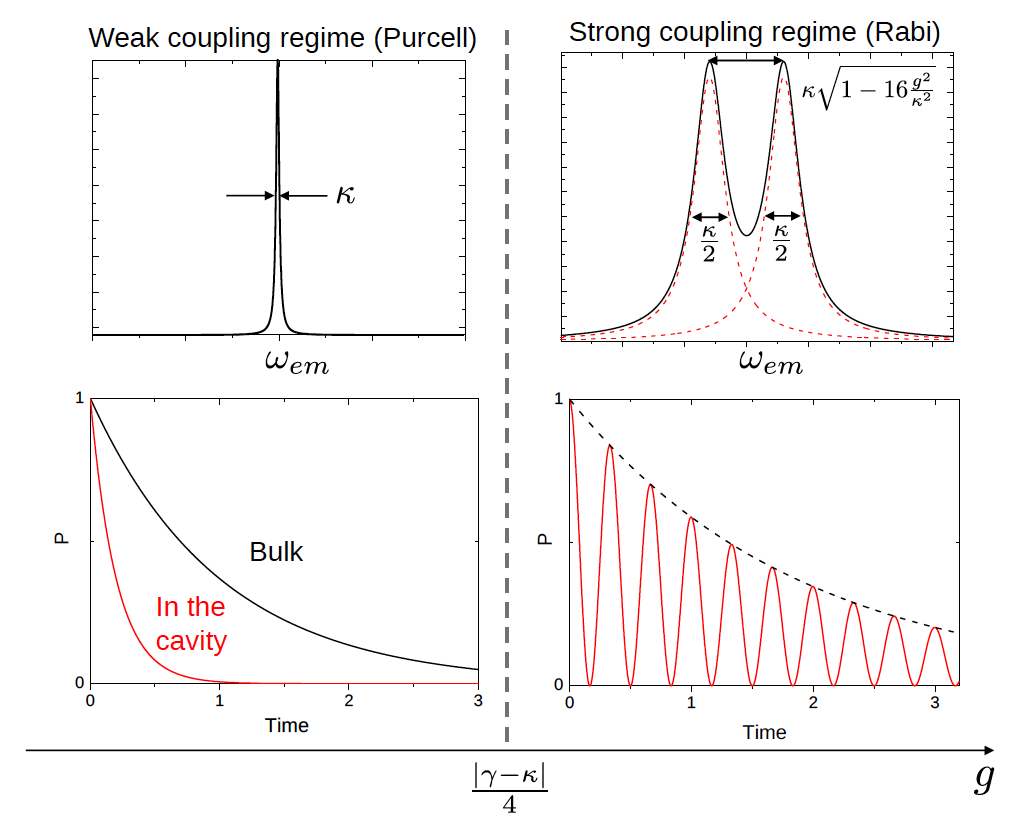
\includegraphics[width=.7\textwidth]{images/Rabi}
\end{figure}
\end{frame}

\begin{frame}{Raman spectroscopy of CNTs}
\begin{figure}
\centering
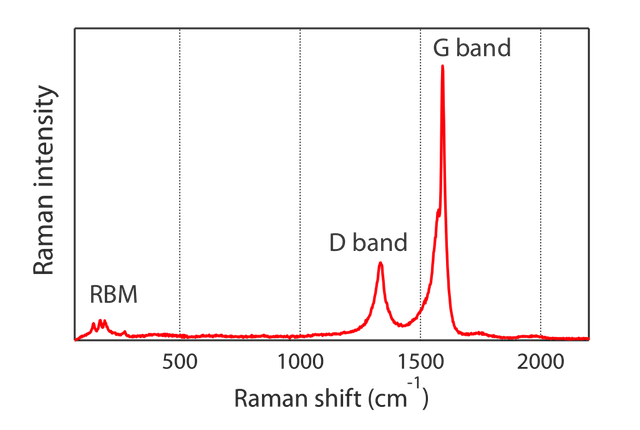
\includegraphics[width=.9\textwidth]{images/raman}
\end{figure}
\end{frame}
\end{document}
